\documentclass[extras,11pt]{article} \usepackage{fullpage}
\usepackage{wrapfig}
\usepackage[T1]{fontenc}
\usepackage{ae,aecompl}
\usepackage{amsmath,amssymb}
\usepackage{amsthm}
\usepackage{hyperref}
\usepackage{calc}
\usepackage{tikz}
\usepackage{bold-extra}
\usepackage{subfigure}
\newtheoremstyle{mytheorem}{\topsep}{\topsep}{\sffamily}{}{\bfseries}{.}{.5em}{}
\theoremstyle{mytheorem}
\newtheorem{theorem}{Theorem}
\newtheorem{claim}[theorem]{Claim}
\newtheorem{lemma}[theorem]{Lemma}
\newtheorem{corollary}[theorem]{Corollary}
\renewenvironment{proof}{\par\noindent{\bf Proof.}\hspace{0.5em}}
    {\hfill\qed\vspace{1ex}}


\newenvironment{proofof}[1]{\par\noindent{\bf #1.}\hspace{0.5em}}
    {\hfill\qed\vspace{1ex}}


\DeclareMathOperator{\poly}{poly}
\DeclareMathOperator{\len}{length}
\DeclareMathOperator{\lev}{level}
\DeclareMathOperator{\comp}{comp}
\newcommand{\eps}{\epsilon}
\newcommand{\prob}[1]{\textit{#1}}
\newcommand{\I}{\mathcal{I}}
\newcommand{\DD}{\mathcal{D}}
\newcommand{\K}{\mathcal{K}}
\newcommand{\PP}{\mathcal{P}}
\newcommand{\C}{\mathcal{C}}
\newcommand{\B}{\mathcal{B}}
\newcommand{\G}{\mathcal{G}}
\newcommand{\eL}{\mathcal{L}}
\newcommand{\pr}{\mathbf{Pr}}
\newcommand{\R}{\mathbb{R}}
\newcommand{\algo}[1]{\textsc{#1}}
\newcommand{\QQ}{{\mbox{\rm\bf Q}}}
\newcommand{\Zplus}{\Z^+}
\newcommand{\Rplus}{{\cal R}^{\geq}}
\newcommand{\OPT}{\mbox{\rm OPT}}
\newcommand{\LP}{\mbox{\rm LP}}
\newcommand{\DLP}{\mbox{\rm D-LP}}
\newcommand{\N}{\mathbb{N}}
\makeatletter\newenvironment{algorithm}{\begin{lrbox}{\@tempboxa}\begin{minipage}{\columnwidth-1cm}}{\end{minipage}\end{lrbox}\centerline{\fbox{\usebox{\@tempboxa}}}
}\makeatother
\newcommand{\algtitle}[1]{\vspace{.1cm}\textbf{#1}}
\newcommand{\alginput}[1]{\\\textbf{Input:} \textit{#1}}
\newcommand{\algoutput}[1]{\\\textbf{Output:} \textit{#1}}
{\makeatletter
 \gdef\xxxmark{\expandafter\ifx\csname @mpargs\endcsname\relax \expandafter\ifx\csname @captype\endcsname\relax \marginpar{xxx}\else
       xxx \fi
   \else
     xxx \fi}
 \gdef\xxx{\@ifnextchar[\xxx@lab\xxx@nolab}
 \long\gdef\xxx@lab[#1]#2{{\bf [\xxxmark #2 ---{\sc #1}]}}
 \long\gdef\xxx@nolab#1{{\bf [\xxxmark #1]}}
}
\begin{document}

\date{}
\title{Euclidean Prize-collecting Steiner Forest\footnote{A short version of this paper appears in Proceedings of LATIN 2010~\cite{BH10:latin}.}}



\author{MohammadHossein Bateni\thanks{Department of Computer Science, Princeton University, Princeton, NJ 08540; Email: \textsf{mbateni@cs.princeton.edu}.
The author was supported by 
a Gordon Wu fellowship as well as
NSF ITR grants
                      CCF-0205594, CCF-0426582 and NSF CCF 0832797,
                      NSF CAREER award CCF-0237113,
                      MSPA-MCS award 0528414,
                      NSF expeditions award 0832797.}
 \and MohammadTaghi Hajiaghayi\thanks{AT\&T Labs---Research, Florham Park, NJ 07932; Email: \textsf{hajiagha@research.att.com}.}}
\maketitle

\begin{abstract}
In this paper, we consider {\em Steiner forest} and its
generalizations, {\em prize-collecting Steiner forest} and {\em
-Steiner forest}, when the vertices of the input graph are points
in the Euclidean plane and the lengths are Euclidean distances.
First, we present a simpler analysis of the polynomial-time
approximation scheme (PTAS) of Borradaile et
al.~\cite{BKM08:euc-for} for the {\em Euclidean Steiner
forest} problem.
This is done by proving a new structural property and
modifying the dynamic programming by adding a new piece of
information to each dynamic programming state. 
Next we develop a
PTAS for a well-motivated case, i.e., the multiplicative case, of
prize-collecting and budgeted Steiner forest.
The ideas used in the algorithm may have applications in design of a broad class of bicriteria PTASs.
At the end, we
demonstrate why PTASs for these problems can be hard in the general
 Euclidean case (and thus for PTASs we cannot go beyond the multiplicative case).
\end{abstract}
\section{Introduction}


Prize-collecting Steiner problems are well-known
 network design problems with several applications in
expanding telecommunications networks (see e.g.~\cite{JMP00,SCRS}),
cost sharing, and Lagrangian relaxation techniques (see e.g.
\cite{JV01,CRW01}). The most general version of these problems is
called the {\em prize-collecting Steiner forest (PCSF)}
problem\footnote{It is sometimes called
{\em prize-collecting generalized Steiner tree (PCGST)} in the literature.}, in which,
given a graph , a set of (commodity) pairs
, a non-negative cost function
, and finally a non-negative penalty
function , our goal is a
minimum-cost way of buying a set of edges and paying the penalty for
those pairs which are not connected via bought edges. When all
penalties are , the problem is the classic APX-hard
\prob{Steiner forest} problem for which the best approximation
factor is  ( is the number of vertices of the
graph) due to Goemans and Williamson~\cite{GW95}. When all sinks are
identical in the PCSF problem, it is the classic prize-collecting
Steiner tree problem. Bienstock, Goemans, Simchi-Levi, and
Williamson~\cite{BGSW93} first considered this problem (based on a
problem earlier proposed by Balas~\cite{Bal89}) for which they gave
a 3-approximation algorithm.
The current best approximation algorithm for this problem is a
recent 1.992-approximation algorithm of Archer, Bateni, Hajiaghayi,
and Karloff~\cite{ABHK09} improving upon a primal-dual
-approximation algorithm of Goemans
and Williamson~\cite{GW95}. When in addition all penalties are
, the problem is the classic \prob{Steiner tree} problem,
which is known to be APX-hard \cite{cr:7} and for which the best
known approximation factor is ~\cite{cr:31}.


  There are several
-approximation algorithms for the \prob{prize-collecting Steiner forest}
problem using LP rounding, primal-dual, or iterative rounding methods which
are first initiated by Hajiaghayi and Jain~\cite{HJ06}
(see~\cite{BGSW93,Hajiagha:iter}).
Currently the best approximation factor for this problem is a
randomized -approximation algorithm \cite{HJ06}. The approach
of Hajiaghayi and Jain has been generalized by Sharma, Swamy, and
Williamson~\cite{SSW07} for network design problems where violating
arbitrary 0-1 connectivity constraints are allowed in exchange for a
very general penalty function.



Lots of attention has been paid to budgeted versions of Steiner problems
as well. In the \prob{-Steiner forest} (or just -forest for
abbreviation), given a graph  and a set of (commodity)
pairs , the goal is to find a minimum-cost forest that connects
at least  pairs of . The best current approximation factor
for this problem is in
~\cite{GHNR07}. On the other
hand, Hajiaghayi and Jain~\cite{HJ06} could transform notorious
\prob{dense -subgraph} to this problem, for which the current best
approximation factor is ~\cite{FKP01}. The
special case in which we have a root  and  consists of all
pairs  for  is the well-known NP-hard
-MST problem. The first non-trivial approximation algorithm for
the -MST problem was given by Ravi et al.~\cite{ch:18}, who
achieved an approximation ratio of . Later this
approximation ratio is improved to a constant by Blum et
al.~\cite{ch:7}. Currently the best approximation factor for this
problem is  due to Garg~\cite{ch:11}.

In this paper, we consider \prob{Euclidean prize-collecting Steiner
forest} and \prob{Euclidean -forest} in which  the vertices of the input graph are
points in the Euclidean plane (or \iffalse in\fi low-dimensional Euclidean
space) and the lengths are Euclidean distances. For the \prob{Euclidean
Steiner tree} problem, Arora~\cite{arora98:ptas} and Mitchell
\cite{cr:26} gave polynomial-time approximation schemes (PTASs).
    Recently Borradaile, Klein and Kenyon-Mathieu~\cite{BKM08:euc-for} claim a PTAS for the
  more general problem of \prob{Euclidean Steiner forest} .







\subsection{Problem definition}


Motivated by the settings in which the demand of each pair is the
product of the weight of the origin vertex and the weight of the
destination vertex in the pair and thus in a sense contributions of
each vertex to all adjacent pairs are the same (e.g., see {\em
product multi-commodity flow} in Leighton and Rao~\cite{LR99} or \cite{Bonsma,KS02}, and
its applications in wireless networks~\cite{MSL08} or
routing~\cite{CKS04,CKS05}), we consider the following multiplicative
version of prize-collecting Steiner forest for the Euclidean case.



In the \prob{Multiplicative prize-collecting Steiner forest
(MPCSF)} problem, given an undirected graph  with
non-negative edge lengths  for each edge , and also
given weights  for each vertex , our goal is to
find a forest  which minimizes the cost

Indeed, this is an instance of PCSF in which each ordered vertex pair
 forms a request with penalty .\footnote{We can change the definition to unordered pairs whose treatment requires only a slight modifications of the algorithms.  Currently, each unordered pair  has a prize of  if .}
 We may be asked
to \emph{collect a certain prize }, in which case the goal is to
find the forest  of minimum cost for which

Let us call this problem -MPCSF. We show that this is a
generalization of the -MST problem (see Appendix~\ref{sec:kmst}) and thus currently there is no approximation better than 2
for this problem either. When working on the Euclidean case, the
input does not include any Steiner vertices, as all the points of
the plane are potential Steiner points.

A bicriteria -approximate solution for the the
-MPCSF problem is one whose cost is at most , yet
collects a prize of at least . Our main contribution in
this paper is a bicriteria -approximation
algorithm that runs in time exponential in  but polynomial
in  and . We then use this  algorithm to obtain a PTAS for
MPCSF.

\subsection{Our contribution}\label{sec:contrib}
First of all, we present a simpler \iffalse\footnote{TODO: how many pages to how many pages?  which lemmas correspond to what?}\fi analysis for the algorithm of
Borradaile et al.~\cite{BKM08:euc-for} for the
\prob{Euclidean Steiner forest} problem and reprove the following
theorem.
\begin{theorem}\label{thm:sf}
 For any constant , there is an algorithm that runs in polynomial time
 and approximates the \prob{Euclidean Steiner forest} problem within  of the
 optimal solution.
\end{theorem}
This is done by modifying the dynamic programming (DP) algorithm so
that instead of storing paths enclosing the \emph{zones} in the
algorithm by Borradaile et al., we use a bitmap to identify a zone.
The modification results in simplification of the structural
property required for the proof of correctness (See
Section~\ref{sec:struct}). We prove this structural property in
Theorem~\ref{thm:locality}. The proof has some ideas similar to
\cite{BKM08:euc-for}, but we present a simpler charging scheme that
has a universal treatment throughout. Next we give an overview of 
the dynamic programming algorithm in Section~\ref{sec:algo}. We have recently come to know that similar simplifications have been independently discovered by
the authors of~\cite{BKM08:euc-for}, too.

Next we extend the algorithm for Euclidean -MPCSF and MPCSF
problems in Section~\ref{sec:multi}.
\begin{theorem}\label{thm:smpcsf}
 For any , there is a bicriteria -approximation algorithm
 for the \prob{Euclidean -MPCSF} problem,
  that runs in time polynomial
 in  and exponential in .
\end{theorem}
Notice that  need not be a constant.
In particular, if all weights are polynomially bounded integers,
we can find in polynomial time a -approximate solution
that collects a prize of at least ; this can be done by picking
 to be sufficiently small ( is still polynomial).
Next we present a PTAS for \prob{Euclidean MPCSF}.
\begin{theorem}\label{thm:mpcsf}
 For any constant , there is a -approximation algorithm
 for the \prob{Euclidean MPCSF} problem,
  that runs in  polynomial time.
\end{theorem}



We also study the case of asymmetric prizes for vertices in which
each vertex  has two types of weights (type one and type two) and the
prize for an ordered pair  is the product of the first type
weight of , i.e., , and the second type weight of , i.e., .
This case is especially interesting because it generalizes the multiplicative
prize-collecting problem when we have two disjoint sets  and
 and we pay the multiplicative penalty only when two vertices,
one in  and the other one in , are not connected (by
letting for each vertex in  the first type weight be its actual
weight and the second type weight be zero and for each vertex in 
the first type weight be zero and the second type weight be its actual
weight.) After hinting on the arising complications, we show how we
can extend our algorithms for this case as well.

\begin{theorem}\label{thm:asym-smpcsf}
 For any , there is a bicriteria -approximation algorithm
 for the \prob{Euclidean Asymmetric -MPCSF} problem,
  that runs in time polynomial
 in  and exponential in . In addition, for any constant , there is a -approximation algorithm
 for the \prob{Euclidean Asymmetric MPCSF} problem,
  that runs in  polynomial time.
\end{theorem}

Indeed, the algorithms in Theorem~\ref{thm:asym-smpcsf} can be
extended to the case in which there are a constant number of
different types of weights for each vertex generalizing the case in
which we have a constant number of disjoint sets and we pay the
multiplicative penalty when two vertices from two different sets are
not connected.
Notice that the case of two disjoint sets already generalizes
the \prob{prize-collecting Steiner tree} problem (by considering  and )
whose best approximation
guarantee is currently .  

At the end, we present in Section~\ref{sec:challenge} why PCSF and
-forest problems can be APX-hard in the general case (and thus
for PTASs we cannot go beyond the multiplicative case). We conclude
with some open problems in Section~\ref{sec:conclusion}. All the
omitted proofs appear in the appendix.




\subsection{Our techniques for the prize-collecting version}
Here, we summarize our techniques for the multiplicative prize collecting Steiner forest algorithms; see Section~\ref{sec:multi}.
In all those algorithms, we store in each DP state extra parameters,
including 
the sum of the weights, as well as the multiplicative prize already collected in each component.
These parameters enable us to carry out the DP update procedure.
Interestingly, the sum and collected prize parameters have their own precision units.

In the asymmetric version, a major issue is that no fixed unit is good for all sum parameters.  
Some may be small, yet have significant effect when multiplied by others.
To remedy this, we use variable units, reminiscent of the floating-point  storage formats (mantissa and exponent).
To the best of our knowledge, Bateni and Hajiaghayi~\cite{BH09:facility} were the first to take advantage of this idea in the context of (polynomial time) approximation schemes.
The basic idea is that a certain parameter in the description of DP states has a large (not polynomial) range,
however, as the value grows, we can afford to sacrifice more on the precision.
Thus, we store two (polynomial) integer numbers, say , where  denotes a variable unit, and  is the coefficient: the actual number is then recovered by .
The conversion between these representations is not lossless, but the aggregate error can be bounded satisfactorily.

In Section~\ref{sec:prize-mpcsf} we consider the problem where the objective is a linear function of penalties paid and the cost of the forest built.
The challenging case is when the cost of the optimal forest is very small compared to the penalties paid.  
In this case, we identify a set of vertices with large penalties and argue they have to be connected in the optimal solution.  
Then, with a novel trick we show how to ignore them in the beginning, and take them into account only after the DP is carried out.


\section{Preliminaries}\label{sec:prelim}
Let  be the total number of terminals and let  be the total length of the optimal solution.
A \emph{bitmap} is a matrix with 0-1 entries.
Two bitmaps of the same dimensions are called \emph{disjoint} if and only if they do not have value one at the same entry.
Consider two partitions   and  over the same ground set.
Then,  is said to be a \emph{refinement} of 
if and only if
any set of  is a subset of a set in , namely .





\begin{figure}[t]
\centerline
{
\subfigure[\label{fig:dissection:1}]{
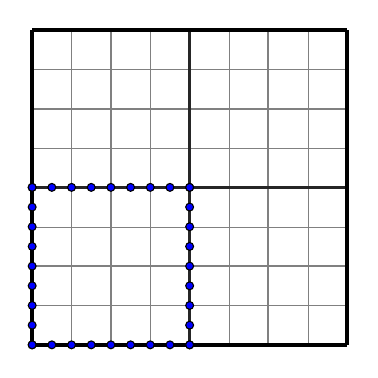
\begin{tikzpicture}
\draw[step=.5cm,gray,ultra thin] (0,0) grid (4,4);
\draw[step=1cm,gray,thick] (0,0) grid (4,4);
\draw[step=2cm,gray!30!black,very thick] (0,0) grid (4,4);
\draw[step=4cm,black,ultra thick] (0,0) grid (4,4);
\foreach \x in {0,1,2,3,4,5,6,7,8}
{
 \draw[fill=blue] (\x*.25,2) circle (.5mm);
 \draw[fill=blue] (\x*.25,0) circle (.5mm);
 \draw[fill=blue] (0,\x*.25) circle (.5mm);
 \draw[fill=blue] (2,\x*.25) circle (.5mm);
}
\end{tikzpicture}
}\hskip 1cm
\subfigure[\label{fig:dissection:2}]{
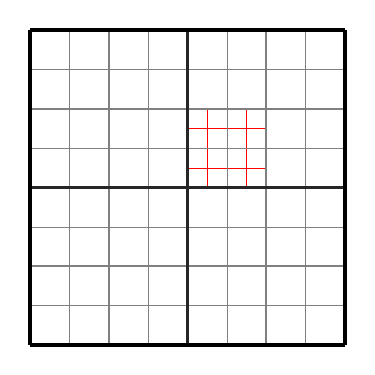
\begin{tikzpicture}
\draw[step=.25cm,red,ultra thin] (2,2) grid (3,3);
\draw[step=.5cm,gray,ultra thin] (0,0) grid (4,4);
\draw[step=1cm,gray,thick] (0,0) grid (4,4);
\draw[step=2cm,gray!30!black,very thick] (0,0) grid (4,4);
\draw[step=4cm,black,ultra thick] (0,0) grid (4,4);
\end{tikzpicture}
}}
\caption{\subref{fig:dissection:1} An example of a dissection square with depth , and depiction of portals for a sample dissection square with ;
\subref{fig:dissection:2} the  grid of cells inside a sample dissection square with .\label{fig:dissection}}
\end{figure}
By standard perturbation and scaling techniques, we can assume the following conditions hold 
incurring a
cost increase of ; see \cite{arora98:ptas,BKM08:euc-for} for example.
\begin{itemize}
\item[(I)] The diameter of the set  is at most .  \item[(II)] All the vertices of  and the Steiner points have coordinates  where  and  are integers.
\end{itemize}
\vspace{-1.5mm}


For simplicity of exposition, we ignore the above increase in cost.
As we are going to  obtain a PTAS, this increase will be absorbed in the future cost increases.
We have a grid consisting of vertical and horizontal lines with equations  and  where  and  are integers.
Let  denote the set of lines in the grid. We let  be the smallest power of two greater than or equal to 
and perform a dissection on the randomly shifted bounding box of size ; see Figure~\ref{fig:dissection:1}.


For each dissection square  and each side  of ,
designate  equally spaced points along  (including the corners) as \emph{portals} of  where  is the smallest power of  greater than .
So the square  has  portals.


There is a notion of \emph{level} associated with each dissection square, line, or side of a square.
The bounding box has level zero, and level of each other dissection square is one more than the level of its parent dissection square.
The level of a line  is the minimum level of a square  a side of which falls on the line .
Thus, the first two lines dividing the bounding box have level one.
If a side  of a square  falls on a line , we define .
So .  The thickness of the lines in Figure~\ref{fig:dissection} denotes their level:
the thicker the line, the lower is its level.

For a (possibly infinite) set of geometric points , let  denote the number of connected components of ;
we will use the shorthand ``component'' in this paper.
With slight abuse of notation,  is used to refer to the set of points\footnote{not necessarily terminals} on .
In addition, we use  to denote the union of points on the lines in .
Similarly, we use  to denote the set of all points on or inside the square .
The set of points on (the boundary of) the square  is referred to by .
The total length of all line segments in  is denoted by .




The following theorem is mentioned in \cite{BKM08:euc-for} in a stronger form.
We only need its first half  whose proof follows from \cite{arora98:ptas}.
\begin{theorem}{\cite{BKM08:euc-for}}
\label{thm:twoprops}
There is a solution  having expected length at most  such that each dissection square  satisfies the following two properties:
for each side  of ,  has at most  non-corner components\footnote{Non-corner components are those not including any corners of squares.  Note that each square can have at most four corner components.} (\emph{boundary components property}); and
each component of  contains a portal of  (\emph{portal property}).
\end{theorem}













\section{Structural theorem}\label{sec:struct}
Let  be a dissection square.
Divide  into a regular  grid of \emph{cells}, where  is a constant power of two determined later; see Figure~\ref{fig:dissection:2}.
We say  is the \emph{owner} of these cells.
The level of these cells, as well as the new lines they introduce, is defined in accordance with the dissection.
That is, we assign them levels as if they are normal dissection squares and we have continued the dissection procedure for  more levels.
There are several lemmas in the work of \cite{BKM08:euc-for} to prove the structural property they require (this is the main contribution of that work).
We modify the dynamic programming definition such that its proof of correctness needs a simpler structural property.
The proof of this property is simpler than that in the aforementioned paper.
\begin{theorem}\label{thm:locality}
There is a solution  having expected length at most  such that each dissection square  satisfies the \emph{locality property}:
if the terminals  and  are inside a cell  of  and are connected to  via ,
 then they are connected in .
\end{theorem}
The proof has ideas similar to \cite[Theorem 3.2, and Lemmas 3.3, 3.4, 3.5 and 3.9]{BKM08:euc-for}.  We first mention and prove a lemma we need in order to prove Theorem~\ref{thm:locality}.
The lemma more or less appears in \cite{arora98:ptas,BKM08:euc-for}.
\begin{lemma}\label{lem:tot-int}
For the forest  output by Theorem~\ref{thm:twoprops},
.
\end{lemma}




We can now prove the main structural result.
A side  of a square  is called \emph{private} if it does not lie on a side of the parent square  of .
Observe that out of any two opposite sides of a dissection square, exactly one is private.

\begin{proofof}{\proofname\ of Theorem~\ref{thm:locality}}
We start with a solution  satisfying Theorem~\ref{thm:twoprops}.
The final solution is produced by iteratively finding the smallest cell  owned  by a square  that violates the locality property,
and adding  to , where  is defined as the union of 
the private sides of 
and
any side of  having non-empty intersection with .
We claim the locality property is realized after finitely many such additions.
If after adding  to , the cell  still violates the locality property, there has to  be exactly two opposite sides of the cell having non-empty intersection with ; otherwise, the  is clearly connected.
However, in case of the opposite sides, one middle side will be a private side of  and hence included as well.

Next, we argue that the conditions of Theorem~\ref{thm:twoprops} still hold.
Take a side  of any square .
If the conditions are to be affected for ,
it has to be due to an addition involving a cell  that has a side  such that
(1)  has non-empty intersection with , and (2)  is added to  as part of .
The condition will be trivial if  contains .
Thus, we assume that  is a smaller square than .
So  cannot be a private side of .
However, the number of components on  cannot increase if  has already an intersection with .


Finally we  show that the additional length is not large.
Let ,
and let  be the set of all grid points.
We will charge the additions to the connected components of .
Notice that

Inequality~\eqref{eqn:2} holds because removal of each grid point on  increases the number of components by at most three.
To obtain \eqref{eqn:3}, notice that in any connected component of ,
the distance between any two points of  is at least .
Hence, if there are more than one such points, there cannot be more than  ones.

We charge this addition to a connected component of ,
 in such a way that each connected component is charged to at most twice: once from each side.
For simplicity, we duplicate each connected component of : they correspond to squares from either side of .
For any dissection square , let   refer to the connected components of  that reach .
Further, let  be the set of connected components of .
When  is  added where  is the owner of ,
there are  components  that become connected.
Any element of  connected via  to a component 
is said to be an \emph{interface} of .
The addition will be charged to a \emph{free} interface of some 
with maximum level. This element will no longer be free
for the rest of the procedure.
We argue this procedure  successfully charges all the additions to appropriate border components.
To this end, we shortly prove the following stronger claim via induction on the number of additions performed.
We call a dissection square  \emph{violated} if the locality property does not hold for a cell  owned by .
\begin{claim}\label{clm:cij}
At all times during the execution of this procedure,
any component  has a free interface,
for each violated square .
As a result, any addition can be charged to a free component.
\end{claim}
The second statement of the claim follows from the first part.
The first part is proved as follows.
The claim clearly holds at the beginning, 
since all interfaces are free, and each component has an interface.
Suppose the addition  is performed and let  be the owner of .
We show any dissection square  will stay fine.
Notice that the size of the squares  for which the addition is performed is increasing in time.
Hence, any dissection square  smaller than  is irrelevant in the statement of the claim, since they cannot be violated.
For  itself, each  has at least one free interface.
One of the interfaces is used, and thus the new component formed by their union has a free interface.
Suppose for the sake of reaching a contradiction that
a component  has no free interface after the addition.
Thus   contains ,
and the charging was not done to a private side of .
Recall that prior to the addition,  is connected to some components of  with at least two free interfaces in .
One of them still remains free.
We charged to the interface of maximum level and it was in .
Hence, the free interface is also in , leading to a contradiction.

Let (the random variable)  denote the number of charges to components on  due to cells  owned by squares  of level .
Independently of the randomness  by the above discussion and Claim~\ref{clm:cij}.
Note the cost of adding  (charged to a component on )
is at most  where  is the side length of .
The total increase due to charges to  is at most  where  is the side length of  the bounding box. Due to the randomization in the dissection, 
we have
; see \cite{arora98:ptas} for instance.
The expected increase in length is thus

\noindent We pick  to be the smallest power of two larger than 
to finish the proof.
\end{proofof}

Therefore, with probability , we have .
In the entire argument, no attempt was made to optimize the parameters.







\section{The algorithm}\label{sec:algo}
A \emph{subsolution} for  is a finite set of line segments 
satisfying conditions of Theorems \ref{thm:twoprops} and \ref{thm:locality},
with the extra property that any terminal  in  is connected via  either to its mate or to .
A \emph{configuration}  for  has two portions:
a set  of pairs  and a partition  whose ground set is , such that
\begin{itemize}
\item  is a subset of portals of ;
\item  is a bitmap of size ;
\item  and  are disjoint if ;
\item the total number of portals, namely , is at most ; and
\item bitmaps  and  are disjoint if .
\end{itemize}
The configuration captures sufficient information about  so as to make it possible to take care of the interaction between  and the outside.
In particular, each pair  describes a connected component of , by specifying the set of portals on its boundary and the set of cells connected to these portals.
Roughly speaking, the partition  tells us which components  and  need to be connected from outside :
 this implies the existence of a pair of terminals that are in  and , respectively, but they are not connected in .
We will see below why this restrictive abstraction does not lose any crucial subsolutions.


We say a subsolution  is \emph{compatible} with a  configuration  if
\begin{enumerate}
\item
for any connected component  of  that intersects ,
 there exists a pair  such that
\begin{itemize}
\item  spans ;
\item each connected component of  contains a portal of ;
\item the bitmap  has value one in the positions corresponding to any cell  containing a terminal  of ; and
\end{itemize}
\vspace{-1mm}
\item
 any terminal pair located in different components  and  of  are either connected via ,
 or  and  are in the same set of .
\end{enumerate}



\subsection{The dynamic programming}


\begin{figure}
\begin{algorithm}
\algtitle{Algorithm \algo{EuclideanSteinerForest}}
\alginput{Set of terminals  in the plane, and set  of pairs of terminals}
\algoutput{A forest  connecting pairs in }
\begin{enumerate}\setlength{\itemsep}{-.00in}
\item Carry out the perturbation and scaling.
\item Let  be smallest power of two larger than , where  is the maximum distance of a pair.
\item Perform a random dissection in the bounding box of side .
\item Place  portals on each side of a dissection square, where  is the smallest power of two larger than  .
\item Solve the base cases  for leaf dissection squares :\\
Go over all possible ways of connecting the portals and the center point.
\item Populate the table  in increasing order of size for :\\
      For any  corresponding to  consisting of :
\begin{enumerate}\setlength{\itemsep}{-.02in}
 \item Go over all configurations  corresponding to .
 \item Build  from the union of all components of  with expanded bitmaps.
 \item Build  from the union of .
 \item If there is a terminal pair  where  and  for ,
\begin{itemize}\setlength{\itemsep}{-.02in}
 \item If there is no bitmap in  (or ) containing the cell containing  (or  respectively), the configuration is bad.
 \item Otherwise, merge the sets corresponding to the appropriate components in .
\end{itemize}
 \item Build  by merging components having the same portals,
  and make appropriate changes to .
 \item Build  by removing portals not on .
 \item If any component with empty portal set has unsatisfied connectivity requirement in , the current configurations are not consistent.
 \item Build  by eliminating components with empty portal set.
 \item If any bitmap contradicts the locality property, these configurations are not consistent.
 \item If the configurations are consistent, update  with .

\end{enumerate}
\item Find the final solution among  where  is the bounding box and  has no unsatisfied requirement.
\item Construct the solution  by recursively following the values from .
\end{enumerate}
\end{algorithm}
\caption{The algorithm for \prob{Euclidean Steiner forest} problem.\label{fig:for-alg}}
\end{figure}

In the dynamic program, we build a table , indexed by configurations for each dissection square .
The goal is to populate this table so that  is the minimum length of a subsolution for  that is compatible with .
First of all, we show that for each , the number of configurations is small.
Consider .
There are at most  pairs in .
For a particular , there are

 options for the set of portals .
The bitmap  has  possibilities.
A crude upper bound of  is trivial for possibilities of .
Thus, the total number will be at most

Theorems \ref{thm:twoprops} and \ref{thm:locality} guarantee the existence of a near-optimal solution all whose subproblems are compatible with a  configuration:
The connected components of  reaching  can be decomposed into disjoint bitmaps
because of Theorem~\ref{thm:locality}.
Theorem~\ref{thm:twoprops} on the other hand ensures each connected component on  contains a portal, and the total number of such components is small.
The details of the DP update, as well as its correctness proof, appears 
below.  







The final solution of the problem is obtained from the minimum  where  is the bounding box, and  of  does not require any connections: i.e., all sets of the partition are singletons.
This would imply all the necessary connections have been made inside .
To actually construct the solution, we need to store additional information in each dynamic programming state indicating which configurations it was last updated from.
It is then straightforward to recursively construct the solution, by taking the union of the pertinent configurations.






Here we show how the dynamic programming table for Euclidean prize-collecting Steiner forest 
is updated from the already-computed values.
And finally we show why the update routine is sound and complete.
The table  is populated in the order of increasing size for .
For a base dissection square , finding the value of  is straightforward.
Notice that there is at most one point (possibly with several terminals collocated) inside .
Depending on whether the mates of those terminals are collocated with them or not, we may need to connect some of them to the boundary .
There are only a constant number of portals in , hence we can go over all the ways to connect them up and find the smallest value.
Note that there cannot be any Steiner point inside .

Now we get to the update rule.
Consider a dissection square  and a corresponding configuration .
Let  for , be the children of  in the dissection.
Take corresponding configurations .
Notice that each cell of  consists of exactly four cells of one .
We can expand a bitmap  of  to a bitmap  of dimensions  for ,
by placing three all-zero bitmaps of dimensions  at appropriate locations around .
We do this in such a way that the portion corresponding to  still points to  inside .
Consider all the components  corresponding to the four subsquares, expand their bitmap, and collect them in .
Merge the partitions  to get .
If there is a terminal pair  where  is in  and  is in a different ,
there should be a component corresponding to each of these in  and , respectively.
Otherwise, these configurations do not correspond to any (valid) subsolution.
Merge the sets corresponding to these components in : i.e., they have to be connected.
Next merge any two components of  if they share a portal, and build .
Further, make appropriate changes in .
Build   by removing from  all portals not on .
Some of these components reach  and some do not, namely those with an empty portal set .
If there is any component with empty portal set that is not  one partition set,
we deem the configurations  as \emph{inconsistent}:
in this case, some components that are required to be connected together do not reach the boundary.
Otherwise, remove all the pairs in  with empty portal set to obtain .
Now, if there is a cell of  whose four constituent cells reach the boundary as more than one connected component, the configurations are not consistent either: this contradicts the property of Theorem~\ref{thm:locality}.
Finally, reduce the dimensions of the bitmaps to  such that a cell of the new bitmap acquires value one if and only if there is a one in one of the positions corresponding to the constituent cells in the original bitmap.
Now,  is said to be consistent with the four configurations  if and only if  contains all the requirements of , i.e.,  is a refinement of , and in addition, there exists a  for any  such that  and .  In case these configurations are consistent,
  will take the minimum of its current value and .
You can refer to Figure~\ref{fig:for-alg} for a summary.




\subsection{Proof of correctness}
Correctness follows from induction on the size of the square  that all dynamic programming states have their intended value.
In particular, we know that there is a near-optimal solution all whose subsolutions are compatible with one configuration.
Hence, these will be computed correctly and give the final solution.
More specifically the following claim holds for all DP states.
\begin{lemma}\label{lem:dp-sf}
A dynamic programming state  ends up having the minimum value corresponding to a solution  of , such that for any dissection square  which is a descendant of  in the dissection tree, the subsolution  of  is compatible with a configuration  for .
\end{lemma}



Now, we are at the position to prove the main Theorem regarding the \prob{Euclidean Steiner forest} problem.
\begin{proofof}{\proofname\ of Theorem~\ref{thm:sf}}
By Lemma~\ref{lem:dp-sf}, the proposed dynamic programming is sound and complete.
There are  DP states.
To solve each non-base state, we go over at most  child states and then perform a polynomial consistency check.
Each base case state is computed in constant time.
Hence, the total algorithm runs in time .
\end{proofof}







\subsection{Highlights of the new ideas}\label{sec:newideas}
Here, we point out the differences between our work and the previous work of \cite{BKM08:euc-for}.
Borradaile et al.\ use closed paths to identify the connected zones of the dissection square.
These paths consist of vertical and horizontal lines and all the break-points are the corners of the cells.
As part of their structural property, they prove that they can guarantee a solution in which these zones can be identified via paths whose total length is at most a constant  times the perimeter of the square .
Then each path is represented by a chain of  of length at most : the three values are used to denote moving one unit forward, or turning to the left or right.  This results in a storage of  which is a constant parameter.
Instead, we use a bitmap of size  to address this issue.
Each zone is represented by a bitmap that has an entry one in the cells of the zone.
The bound that we obtain, , may be slightly worse than the previous work, however,
a simpler structural property, namely the locality property, suffices as the proof of correctness.
Borradaile et al.\ in contrast need a bound on the total length of the zone boundaries, as noted above.

In addition to the simplification made due to this change,
both to the proof and the treatment of the dynamic programming,
we simplify the proof further.
Borradaile et al.\ charge the additions of  to three different structures,
and the argument is described and analyzed separately for each.
We manage to perform a universal treatment and charging all the additions to the simplest of the three structures in their work.
But this can be done only  after showing  has a limited number of components.
The proof is simple yet elegant---a weaker claim is proved in \cite{BKM08:euc-for}, but even the statement of the claim is hard to read.

\iffalse
\begin{wrapfigure}{R}[.5cm]{0cm}
{
\subfigure[\label{fig:counter:1}]{
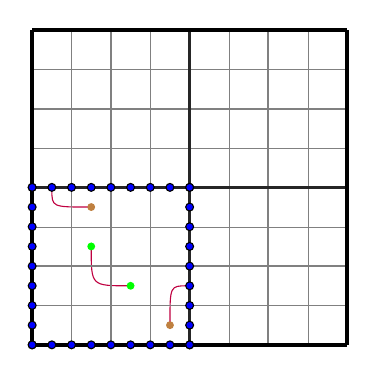
\begin{tikzpicture}
\draw  (.75,1.75) node[inner sep=0mm] (p1) {};
\draw  (1.75,.25) node[inner sep=0mm] (p2) {};
\draw  (.75,1.25) node[inner sep=0mm] (p3) {};
\draw  (1.25,.75) node[inner sep=0mm] (p4) {};
\draw (.25,2) node[inner sep=0mm] (p5) {};
\draw (2,.75) node[inner sep=0mm] (p6) {};
\draw[purple] (p1) .. controls ++(-.5,0) .. (p5);
\draw[purple] (p2) .. controls ++(0,.5) .. (p6);
\draw[purple] (p3) .. controls ++(0,-.5) .. (p4);
\fill[fill=brown]   (p1)  circle (.5mm);
\fill[fill=brown]   (p2)  circle (.5mm);
\fill[fill=green]   (p3)  circle (.5mm);
\fill[fill=green]   (p4)  circle (.5mm);
\draw[step=.5cm,gray,ultra thin] (0,0) grid (4,4);
\draw[step=1cm,gray,thick] (0,0) grid (4,4);
\draw[step=2cm,gray!30!black,very thick] (0,0) grid (4,4);
\draw[step=4cm,black,ultra thick] (0,0) grid (4,4);
\foreach \x in {0,1,2,3,4,5,6,7,8}
{
 \draw[fill=blue] (\x*.25,2) circle (.5mm);
 \draw[fill=blue] (\x*.25,0) circle (.5mm);
 \draw[fill=blue] (0,\x*.25) circle (.5mm);
 \draw[fill=blue] (2,\x*.25) circle (.5mm);
}
\draw[draw=violet] (p3) ++(.2cm,.15cm) node {};
\draw[draw=violet] (p4) ++(.1cm,.2cm) node {};
\draw[draw=violet] (.5cm,1.5cm) node {};
\draw[draw=violet] (1.5cm,1.5cm) node {};
\draw[draw=violet] (.5cm,.5cm) node {};
\draw[draw=violet] (1.5cm,.5cm) node {};
\end{tikzpicture}
}\hskip.2cm
\subfigure[\label{fig:counter:2}]{
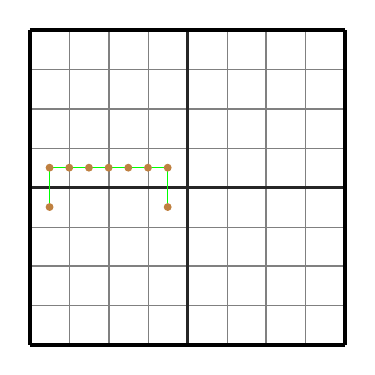
\begin{tikzpicture}
\draw[step=.5cm,gray,ultra thin] (0,0) grid (4,4);
\draw[step=1cm,gray,thick] (0,0) grid (4,4);
\draw[step=2cm,gray!30!black,very thick] (0,0) grid (4,4);
\draw[step=4cm,black,ultra thick] (0,0) grid (4,4);
\draw[draw=green] (.25,1.75) -- (.25,2.25) -- (1.75,2.25) -- (1.75,1.75);
\foreach \x in {1,2,3,4,5,6,7}
 {  \fill[fill=brown] (\x*.25,2.25) circle (.5mm); }
\fill[fill=brown] (.25,1.75) circle (.5mm);
\fill[fill=brown] (1.75,1.75) circle (.5mm);
\end{tikzpicture}
}}
\caption{Problematic example for Borradaile et al.'s DP approach: \subref{fig:counter:1} an example in which we lose the information about a terminal pair's having already been satisfied or not; \subref{fig:counter:2} an example that proves the additional cell property need not be true.\label{fig:dp-counter}}\vskip-0mm
\end{wrapfigure}
The most important change, however, is a bug fix.
Borradaile et al.\ do not provide details of how to populate the DP  table.
We believe that the information they store in the configurations is not sufficient for updating the table.
We add a new piece of information, namely the partition , that addresses this very issue.
Figure~\ref{fig:dp-counter} depicts a problematic example.
Let  be the dissection square in Figure~\ref{fig:counter:1} that has portals on its boundary.
Name the subsquares as  from top to bottom, and left to right.
Notice that a terminal pair  where  and  are connected to each other.
The two other terminals shown in Figure~\ref{fig:counter:1} are connected to the portals and reported through the configurations to the outside.
Observe that the connected component of  and  will not be reported outside, as they do not reach the portals of .
As we move up the dissection tree, we get to a point that  and  each becomes a cell.
At that point, we cannot distinguish between the cases where  and  are connected or not.
One may suggest we could enforce that everything inside the corresponding cells should have been connected.
Remember that the locality property is slightly weaker: only the components reaching  are guaranteed to be connected.
However, in this example, terminals  and  are connected and need not reach the boundary.

We show in Figure~\ref{fig:counter:2} that the stronger property is not always true.
There are two terminals (they form a pair) in the bottom square,
and their distance to the border is very small, say .
The top square contains many terminals such that consecutive terminals have distance .
In addition, the sides of the squares are one unit.
An optimal solution connects the terminals as shown paying a cost of about one unit.
However, if we enforce that the bottom terminals need to be connected, the cost will be about two units.
\xxx{think more about this, is this really a problem?}
\fi







\section{Multiplicative prizes}\label{sec:multi}

We first tackle the \prob{-multiplicative prize-collecting Steiner forest} problem.
Then, we will take a look at its asymmetric generalization.
Finally, we show how the \prob{multiplicative prize-collecting Steiner forest} problem can be reduced to -MPCSF.

\subsection{Collecting a fixed prize}
\label{sec:smpcsf}

Suppose we are given , the amount of prize we should collect.
Let  be the minimum cost of a forest  that collects a prize of at least ,
and suppose  is the set of terminal pairs connected via .
We show how to find a forest with cost at most   that collects
a prize of at least .
By the structural property, we know that there is a solution  connecting the same
 set of terminal pairs  whose cost is at most , yet it satisfies the
 conditions of Theorems~\ref{thm:twoprops} and \ref{thm:locality}.
Round all the vertex weights down to the next integer multiple of
.
In a connected component of  of total weight  that  lost a weight  due to
rounding, the lost prize is ,
because the total weight of the component is at most .
Thus,  collects at least  from the rounded weights.





Each dynamic programming state consists of a dissection square ,
a set of components , and a new parameter 
which denotes the total prize collected inside  by connecting
the terminal pairs.
Each element of ---corresponding to a connected component in the subsolution---now has the form 
where  denotes the portals of , 
and  is the total sum of the weights in .
The DP is carried out in a fashion similar to that of \cite{arora98:ptas}.
The values of  and  are easy to determine for the base cases.
It is not difficult to update them, either.
Whenever two components  and 
merge in the DP, the sum  for the new component is simply .
Besides, the merge increases the  value of the DP state by .



\iffalse
Each dynamic programming state consists of a dissection square , a configuration
, and a new parameter  which denotes the total
 prize collected inside  by connecting the terminal pairs.
In addition, each element of  now has the form ,
where  is the total sum of the weights in .
The values of  and  are easy to determine for the base cases.
It is not difficult to update them either.
Whenever two components  and 
merge in the DP, the sum  for the new component is simply .
Besides, the merge increases the  value of the DP state by .
\fi



\begin{proofof}{\proofname\ of Theorem~\ref{thm:smpcsf}}
The soundness and completeness is simple and is along the same lines as the proof of Theorem~\ref{thm:sf}.
Carrying out the above operation assumes the values of  and  could be stored
accurately.  However, as they describe the dynamic programming states, their size should be
sufficiently small or else the algorithm will not run in polynomial time.
Here does the rounding help us.
All values of  are stored as multiples of  and the values of  are stored
as multiples of .  Notice that as we round the vertex weights at the beginning,
throughout the algorithm the values of  and  will be multiples of their respective
units.  Hence, no extra precision error will occur and we find the aforementioned solution.
If at any time during the execution of the algorithm, the value of  goes above ,
we truncate it to .  Similarly, the value of  is not allowed to surpass .
This does not eliminate any solution, because at the point of truncation, the subsolution has
already gathered sufficient prize.
Hence, the range of  is from zero up to , and this gives
 different values.
Similarly for , there are at most  options.
There are at most

\noindent DP states for each square .
The running time is polynomial in  and the claim follows.
\end{proofof}

To start the algorithm, we need to guarantee the instance satisfies
the conditions at the beginning of Section~\ref{sec:prelim}.
See Appendix~\ref{sec:prelim-mult} for details of how this is achieved.



\subsection{The asymmetric prizes}



The basic idea is to store two parameters  and  for each component of .
These parameters store the total weight of the first and second type in the component, namely  and , respectively.
The difficulty is that to collect a prize of  in a component,
only one of the parameters  or  needs to be large.
In particular, we cannot do a rounding with a precision like .
It may even happen that   is large in one component, whereas we have a large  in another.
In fact, we cannot store the values of the   or  as multiples of a fixed unit.
To get around the problem,  is stored as a pair , where  is  a vertex of the graph
and  is an integer.
Together they show that  is ;
the value of  will be chosen later, and  is supposed to be the vertex of largest
type-one weight present in the component.
A similar provision is made for .
Finally, the value of  is stored as a multiple of ;
we will shortly pick the value of .


Whenever  and  are added to give
,  we do the calculation as follows:
let  be the vertex   or  that has the larger  value,
and then 




\begin{proofof}{\proofname\ of Theorem~\ref{thm:asym-smpcsf}}
The precision error for  is at most
, because there is an accumulation of at most 
rounding errors each of which has been less than .
Notice that if  is stored in terms of the vertex , it has to include  and
thus its type one weight is at least .  Hence, the precision error is at most a
 multiplicative factor.
Therefore, when we do a multiplication of  to get an addition to ,
the error is at most a multiplicative :
.
Next a rounding error may happen to store the value in terms of .
Each  on the other hand is made up of at most  addition terms,
so the total error is at most .
We pick  to conclude that the total error is bounded by
.

All the discussion applies to  as well.
Due to truncation and rounding, there are at most  options for .
And each  (or ) has at most  possibilities.
Thus, the total number of DP states for each dissection square is .
Therefore, we obtain a bicriteria approximation to the asymmetric variant of the problem.
\end{proofof}


\subsection{The prize-collecting version: trade-off between penalty and forest cost}\label{sec:prize-mpcsf}

In the prize-collecting variant, we pay for the cost of the forest,
and for the prizes not collected.
If the total weight is ,
the prize not collected is  minus the collected prize.
One difficulty here is to determine the correct range for the collected prize
so that we can use the algorithm of Section~\ref{sec:smpcsf}.
The trivial range is zero to .
However, the rounding precision we pick for the penalties should also take into
account the cost of the forest.  If the cost of the intended solution is much smaller than
, we cannot simply go with rounding errors like .
Otherwise, the error caused due to rounding the penalties will be too large compared to the solution value.

The trick is to find an estimate of the solution value, and then consider two cases depending on
how the cost compares to the total penalty.
Using a -approximation  algorithm, we obtain a solution of value .
We are guaranteed that .
If ,
 the optimum solution is to collect no prize at all.
Otherwise, assume .
To beat the solution of value , we should collect
a prize of at least .


We first consider the simpler case when :
For an  whose precise value will be fixed below,
we use the algorithm of Section~\ref{sec:smpcsf} to find
a bicriteria -approximate solution for collecting
a prize ; this is done for any  which is a multiple of 
in range .
We select the best one after adding the uncollected prize to each
of these solutions.
Suppose the optimal solution  collects a prize .
Let  be the length of the forest.
Round  down to the next multiple of , say .
Fed with prize value , the algorithm finds a solution that collects
a prize of at least  with forest cost at most .
\begin{claim}\label{clm:mpcsf:eps}
The total cost of this solution is at most  if .
\end{claim}

\begin{proof} The total cost of this solution is

where \eqref{eqn:14} follows from ,
and \eqref{eqn:15} uses the definition of .
\end{proof}





The other case, i.e., , is more challenging.
Notice that in order to carry out the same procedure in this case,  may not be bounded by  and thus the running time may not be polynomial.
The solution, however, has to collect almost all the prize.
Thus, one of the connected components includes almost all the vertex weights.
We set aside a subset  of vertices of large weight.
The vertices of  have to be connected in the solution, or else the paid penalty will be too large. Then, dynamic programming proceeds by ignoring the effect of these vertices and only keeping tabs on how many vertices from  exist in each component.
At the end, we only take into account the solutions that gather \emph{all} the vertices of  in one component and compute the actual cost of those solutions and pick the best one.
In the following, we provide the details of our method and prove its correctness.

Let  be the set of all vertices whose weight is larger than .
\begin{lemma}\label{lem:large-comp}
All the vertices of  are connected in the optimal solution.
\end{lemma}
\begin{proof}
  There are at most  components, so there is a component, say ,
 whose total weight is not less than .
  We claim all the vertices of  are inside this component.
  The penalty paid by the optimal solution is at most .
  If there is any vertex of  outside , the penalty of
 the solution is more than ,
 yielding a contradiction.
\end{proof}

Next, we round up all the weights to the next multiple of 
for vertices not in .
 Define  as the optimal solution of the resulting instance.
 Let  be the length of the forest in , and define  similarly.
 Let  and  denote the penalty paid by  and , respectively.
Assume that .
\begin{lemma}\label{lem:round-err}
.
\end{lemma}
\begin{proof} We recompute the penalties paid by 
 using the rounded weights.
 The pair  not connected in   is either of the two kinds:
 (1) one of  and  is in ; or (2) none of them is in .
 The total rounding error for the penalties of the first type is bounded by
 .
 There are at most  pairs of the second type.
  Since the weights of these terminals are at most ,
 the error is not more than .
 Hence, the total error is at most

which is no more than  as desired.
\end{proof}






Suppose we use a dynamic programming approach similar to the previous subsections
to find the approximately minimum forest length for any specified collected prize amount;
in particular, we obtain a bicriteria -approximate solution.
During this process, we ignore the weights associated with vertices in .
Consider a DP state  corresponding to a dissection square .
Each component  looks like  :
the new piece of information, , is an integer number denoting the number of
vertices of  inside .
Extending the previous algorithm to populate the new DP table is simple.
Finally, we look at all the configurations  for the bounding box such that
the  value of one component is exactly  whereas it is zero for all other components.
This guarantees that all elements of  are inside the former component and hence
we can add up the penalties involving those vertices.
Let  where ,
and let  be the component containing .
The additional cost due to vertices of  is

Finally, we report the best solution corresponding to these configurations.


\begin{proofof}{\proofname\ of Theorem~\ref{thm:mpcsf}}
Let us first see that the algorithm described runs in polynomial time.
It is sufficient to bound the number of configurations.
The new piece of information has at most  possibilities.
Further,  is always a multiple of .
Similarly,  will not exceed  and is always a multiple of .

 We pick .
  By Lemmas~\ref{lem:large-comp} and \ref{lem:round-err}, the rounding does not increase the penalties paid by the optimal solution by more than .
 We then utilize the algorithm described for -MPCSF to find a solution of cost at most .
Finally,  changing the weights back to the original values clearly does not increase the cost.
\end{proofof}






\section{Evidence for Hardness}\label{sec:challenge}

So far PTASs for geometric problems in Euclidean plane including
ours and those of Arora \cite{arora98:ptas} and Mitchell
\cite{cr:26} can be easily generalized for Euclidean -dimensional
space, for any constant . However we can prove the following
theorem on the hardness of the problem for Euclidean -dimensional
space.

\begin{theorem}
If notorious densest -subgraph is hard to approximate within a
factor  for some constant , then for any , the -forest problem in Euclidean -dimensional space is
hard to approximate within a factor
.
\end{theorem}
\begin{proof}
Hajiaghayi and Jain~\cite{HJ06} show that if densest -subgraph is
hard to approximate within a factor , then the
-forest problem on stars is hard to approximate within a factor
. On the other hand, Gupta~\cite{Gupta00} shows
that a tree metric of size  can be embedded into Euclidean
-dimensional space with distortion in .
Thus for any , we cannot obtain an approximation factor
 for -forest in Euclidean
-dimensional space, since otherwise by solving the problem in
Euclidean -dimensional space, finding an Eulerian tour and
shortcutting it, and finally embedding it back into the star, we can
obtain a better approximation than , a
contradiction.
\end{proof}


Note as mentioned above that, despite extensive study, 
the current best approximation factor 
for notorious densest -subgraph is
~\cite{FKP01} and thus we do not expect
to have any PTAS for -forest in -dimensional Euclidean space.



Unlike the general cases of these problems,
 as far as PTASs for the case of Euclidean spaces are concerned,
 it seems \prob{-forest} and \prob{prize-collecting Steiner forest} problems are essentially equivalent.
 Indeed in Lemma~\ref{lem:kfor>pcsf}, we prove that any PTAS for \prob{-forest} results in a PTAS for \prob{prize-collecting Steiner
 forest},
 and we believe that any DP algorithm giving a PTAS for PCSF computes
 along its way the optimal solution to different -forest instances.


Thus based on the evidences above, we do believe \prob{Euclidean
-forest} and \prob{Euclidean prize-collecting Steiner forest}
have no PTASs in their general forms.






\section{Conclusion}
\label{sec:conclusion} Besides presenting a simpler and correct
analysis of the PTAS for the \prob{Euclidean Steiner forest
problem}, we showed how the approach can be generalized to solve
multiplicative prize-collecting problems.



Generalizing our results to planar graphs, especially obtaining a
PTAS for Steiner forest, has been a long-standing open problem in this field.
The question was settled very recently by Bateni, Hajiaghayi and Marx~\cite{BHM09:forest}.
While Borradaile, Klein and Kenyon-Mathieu~\cite{BKM07} gave a
PTAS for \prob{Steiner tree} on planar graphs, a main ingredient
of their algorithm is solving \prob{Steiner tree} on graphs of
bounded-treewidth. However in a sharp contrast, Gassner~\cite{Gas08}
showed recently that \prob{Steiner forest} is NP-hard even on graphs of
treewidth at most 3.
Bateni et al.~\cite{BHM09:forest} 
gives a PTAS for the problem on graphs of bounded treewidth,
and uses it to obtain a PTAS for planar and bounded-genus graphs.


Last but not least, obtaining any improvement over the approximation
factor 2.54 in~\cite{HJ06} for multiplicative prize-collecting
Steiner forest in general graphs seems very interesting.




{\bibliographystyle{siam} \bibliography{main2}
}














\appendix



\iffalse

\section{Dynamic programming details}\label{sec:dp-details}

Here we show how the dynamic programming table for Euclidean prize-collecting Steiner forest 
is updated from the already-computed values.
And finally we show why the update routine is sound and complete.
The table  is populated in the order of increasing size for .
For a base dissection square , finding the value of  is straightforward.
Notice that there is at most one point (possibly with several terminals collocated) inside .
Depending on whether the mates of those terminals are collocated with them or not, we may need to connect some of them to the boundary .
There are only a constant number of portals in , hence we can go over all the ways to connect them up and find the smallest value.
Note that there cannot be any Steiner point inside .

Now we get to the update rule.
Consider a dissection square  and a corresponding configuration .
Let  for , be the children of  in the dissection.
Take corresponding configurations .
Notice that each cell of  consists of exactly four cells of one .
We can expand a bitmap  of  to a bitmap  of dimensions  for ,
by placing three all-zero bitmaps of dimensions  at appropriate locations around .
We do this in such a way that the portion corresponding to  still points to  inside .
Consider all the components  corresponding to the four subsquares, expand their bitmap, and collect them in .
Merge the partitions  to get .
If there is a terminal pair  where  is in  and  is in a different ,
there should be a component corresponding to each of these in  and , respectively.
Otherwise, these configurations do not correspond to any (valid) subsolution.
Merge the sets corresponding to these components in : i.e., they have to be connected.
Next merge any two components of  if they share a portal, and build .
Further, make appropriate changes in .
Build   by removing from  all portals not on .
Some of these components reach  and some do not, namely those with an empty portal set .
If there is any component with empty portal set that is not  one partition set,
we deem the configurations  as \emph{inconsistent}:
in this case, some components that are required to be connected together do not reach the boundary.
Otherwise, remove all the pairs in  with empty portal set to obtain .
Now, if there is a cell of  whose four constituent cells reach the boundary as more than one connected component, the configurations are not consistent either: this contradicts the property of Theorem~\ref{thm:locality}.
Finally, reduce the dimensions of the bitmaps to  such that a cell of the new bitmap acquires value one if and only if there is a one in one of the positions corresponding to the constituent cells in the original bitmap.
Now,  is said to be consistent with the four configurations  if and only if  contains all the requirements of , i.e.,  is a refinement of , and in addition, there exists a  for any  such that  and .  In case these configurations are consistent,
  will take the minimum of its current value and .
You can refer to Figure~\ref{fig:for-alg} for a summary.



\begin{figure}
\begin{algorithm}
\algtitle{Algorithm \algo{EuclideanSteinerForest}}
\alginput{Set of terminals  in the plane, and set  of pairs of terminals}
\algoutput{A forest  connecting pairs in }
\begin{enumerate}\setlength{\itemsep}{-.00in}
\item Carry out the perturbation and scaling.
\item Let  be smallest power of two larger than , where  is the maximum distance of a pair.
\item Perform a random dissection in the bounding box of side .
\item Place  portals on each side of a dissection square, where  is the smallest power of two larger than  .
\item Solve the base cases  for leaf dissection squares :\\
Go over all possible ways of connecting the portals and the center point.
\item Populate the table  in increasing order of size for :\\
      For any  corresponding to  consisting of :
\begin{enumerate}\setlength{\itemsep}{-.02in}
 \item Go over all configurations  corresponding to .
 \item Build  from the union of all components of  with expanded bitmaps.
 \item Build  from the union of .
 \item If there is a terminal pair  where  and  for ,
\begin{itemize}\setlength{\itemsep}{-.02in}
 \item If there is no bitmap in  (or ) containing the cell containing  (or  respectively), the configuration is bad.
 \item Otherwise, merge the sets corresponding to the appropriate components in .
\end{itemize}
 \item Build  by merging components having the same portals,
  and make appropriate changes to .
 \item Build  by removing portals not on .
 \item If any component with empty portal set has unsatisfied connectivity requirement in , the current configurations are not consistent.
 \item Build  by eliminating components with empty portal set.
 \item If any bitmap contradicts the locality property, these configurations are not consistent.
 \item If the configurations are consistent, update  with .

\end{enumerate}
\item Find the final solution among  where  is the bounding box and  has no unsatisfied requirement.
\item Construct the solution  by recursively following the values from .
\end{enumerate}
\end{algorithm}
\caption{The algorithm for \prob{Euclidean Steiner forest} problem.\label{fig:for-alg}}
\end{figure}



\subsection{Proof of correctness}
Correctness follows from induction on the size of the square  that all dynamic programming states have their intended value.
In particular, we know that there is a near-optimal solution all whose subsolutions are compatible with one configuration.
Hence, these will be computed correctly and give the final solution.
More specifically the following claim holds for all DP states.
\begin{lemma}\label{lem:dp-sf}
A dynamic programming state  ends up having the minimum value corresponding to a solution  of , such that for any dissection square  which is a descendant of  in the dissection tree, the subsolution  of  is compatible with a configuration  for .
\end{lemma}



Now, we are at the position to prove the main Theorem regarding the \prob{Euclidean Steiner forest} problem.
\begin{proofof}{\proofname\ of Theorem~\ref{thm:sf}}
By Lemma~\ref{lem:dp-sf}, the proposed dynamic programming is sound and complete.
There are  DP states.
To solve each non-base state, we go over at most  child states and then perform a polynomial consistency check.
Each base case state is computed in constant time.
Hence, the total algorithm runs in time .
\end{proofof}

\fi





\section{Deferred proofs and further discussion}

\begin{proofof}{\proofname\ of Lemma~\ref{lem:tot-int}}
 The proof of Theorem~\ref{thm:twoprops} (although not reproduced here) does not increase .
 Hence, it suffices to prove the result for the forest  specified at the beginning of Section~\ref{sec:prelim}.
 Observe that by (II),   consists merely of singleton points,
 because no Steiner point lies on a line .
 Further notice that the -length of  is at most .
 Let  be the total absolute distance  travels in the  direction. Since -coordinate difference of any two consecutive \emph{break-points} of  is a multiple of  and the intersection with vertical lines of  occurs at coordinates of the form , the total number of intersections with vertical lines is exactly .
 We can similarly argue for the intersections with horizontal lines, and finally conclude that  .
\end{proofof}


\begin{proofof}{\proofname\ of Lemma~\ref{lem:dp-sf}}
This is clearly true for the base cases of the DP since we go over all the possibilities.
Next, take any configuration  corresponding to a non-leaf dissection square ,
and suppose there is a subsolution  with respect to  compatible with ,
 such that any subsolution  formed by restricting  to a dissection square  which is a descendant of  is compatible with some configuration  of .
Let  be the subsolutions restricted to the subsquares .
Each of them is thus compatible with an appropriate .
By inductive hypothesis, the dynamic programming states  have been correctly computed.
Each connected component of  not connected to  has to have all its terminal pairs satisfied.
This is taken care of by checking the partition :
the terminals in components that do not advance in the dynamic table to  have their demands satisfied internally.
In addition, the locality property for  ensures the configurations will be consistent,
and hence we perform an update of  from .
This finishes the completeness proof.

Verifying that the update rule is sound is trivial.
If the four configurations  update ,
then there exists a subsolution  formed by the union of the corresponding subsolutions , that is compatible with .
\end{proofof}


\iffalse
\begin{proofof}{\proofname\ of Claim~\ref{clm:mpcsf:eps}}
The total cost of this solution is

where \eqref{eqn:14} follows from ,
and \eqref{eqn:15} uses the definition of .
\end{proofof}
\fi


\iffalse
\begin{proofof}{\proofname\ of Lemma~\ref{lem:round-err}}
 We recompute the penalties paid by 
 using the rounded weights.
 The pair  not connected in   is either of the two kinds:
 (1) one of  and  is in ; or (2) none of them is in .
 The total rounding error for the penalties of the first type is bounded by
 .
 There are at most  pairs of the second type.
  Since the weights of these terminals are at most ,
 the error is not more than .
 Hence, the total error is at most

which is no more than  as desired.
\end{proofof}
\fi



\subsection{The preliminary conditions for multiplicative prizes}\label{sec:prelim-mult}
In Section~\ref{sec:prelim}, we said that standard perturbation and scaling techniques allow us to assume
with a cost increase of at most 
that the bounding box of the instance has side length at most ,
while restricting all vertices and Steiner points to points of the form  for integers  and .
The claim is based on the following two premises:
\begin{enumerate}\setlength{\itemsep}{-.01in}
\item If  is the maximum distance of a pair in , then .
\item If  and 
are farther than ,
they cannot be connected in the optimum solution.
\end{enumerate}
Using this, the instance can be broken up into disjoint subinstances and then the perturbation can be carried out.
However, the first premise is false in the case of multiplicative prizes since not all the pairs need to be connected.
Next we show how similar conditions can be guaranteed in this case.

The value of  can be \emph{guessed} using binary search.
To begin the search, we can get crude bounds of ,
using simple approximation algorithms for the general cases of PCSF and -forest.\footnote{The best known approximation algorithms known for these problems are  and , respectively.}
Knowing , we build a graph  on the vertices:
there is an edge between  and  if and only if their distance is at most .
The diameter of each connected component is at most .
We consider each of them separately, since two vertices in different components cannot be connected in the optimal solution.

The side length of the bounding box is at most .
Scale the instance by  and let  denote the new optimal value.
Build a grid in the bounding by lines with equations  and  for integers .
Move each vertex and Steiner point to the closest point of the form .
Notice that there are at most  Steiner points.
Assuming , the change in the solution value
due to the perturbation is at most .
Hence, we can assume that
\begin{itemize}\setlength{\itemsep}{-.01in}
\item the side length of the bounding box is at most , and
\item the vertices and Steiner points are at coordinates  for integers .
\end{itemize}





\subsection{-MST as a special case of -MPCSF}\label{sec:kmst}
Here we show that (even the symmetric) -MPCSF is a generalization of the rooted -MST problem (for which the best approximation guarantee is ).
Suppose we are given an instance  of the rooted -MST problem.
It consists of a graph , edge lengths , a root vertex  and a number .
Suppose  is not to be counted among the  vertices.
We build the new instance  of the -MPCSF problem as follows.
The graph  is the same as .
The weights of all vertices are one, except for  whose weight is .
Then, the goal will be to find the cheapest forest that gathers a prize of at least .

\begin{theorem}\label{thm:special-case}
The instance  of the rooted -MST problem
is equivalent to
the instance  of the -MPCSF problem.
\end{theorem}
\begin{proof}
As we noted in Subsection~\ref{sec:contrib},
in case of polynomially bounded integer weights,
we can make sure the returned solution collects a prize of at least  (without any approximation factor).
This can be achieved by picking .

Obviously, any tree connecting  vertices to the root is translated
to a forest that collects a prize of at least .
Let each vertex not spanned by the tree be a singleton component in the forest.

Finally, we claim that any solution of value  or higher translates to a solution of value at least  for the original instance.
The resulting tree is just the component of the forest containing the root vertex.
Suppose for the sake of reaching a contradiction that the component spans  non-root vertices.
The total prize collected is at most

yielding a contradiction, and proving the supposition is false.
\end{proof}









\subsection{PCSF vs. -forest}
\begin{lemma}\label{lem:kfor>pcsf}
 An -approximation algorithm for the \prob{-forest} problem
 gives an -approximation algorithm for the \prob{prize-collecting Steiner forest} problem, for any constant .
\end{lemma}
\begin{proof}
 We show how to approximate a PCSF instance  by
 invoking several (polynomially many) instances  of the -forest problem.
 Obtain an estimate  for  ,
 such that  using a general-case -approximation algorithm.
 Let  be the penalty of the pair  in .
 Without loss of generality, we can assume that  for any pair .
Let .
 Place  copies  of  the pair  in . Find an -approximate solution to the resulting -forest instance
 for every value of , where  is the number of pairs in .
 Compute the PCSF value for each of these solutions and report the best one.

 We show that at least one of these candidate solutions is good.
 Let  and  be the length of the forest and the paid penalty
 of the optimal solution, respectively.
 Suppose  connects a subset of terminal pairs .
 Then, .
 Focus on the candidate solution with .
 The length of the corresponding -forest instance is
 at most , because a possible solution is that of connecting the copies of  .
 To compute the PCSF value, we add the penalty of pairs in  that are not connected using this tree.
 We can assume either all or no copies of each pair is connected.
 The number of pairs not connected is at most ,
 and  their penalties sum to no more than

Thus, the PCSF value of the best candidate solution is at most .
 It remains to show the instances  have polynomial size.
 Since , each pair  will have  copies.
 Hence,  has polynomial size and we can use the approximation algorithm for the -forest.
\end{proof}











\iffalse

\subsection{-RBSF}\label{sec:krbsf}






\begin{lemma}\label{lem:krbsf->kfor}
An instance of -RBSF can be reduced to an instance of -forest
if the optimal solution to the instance costs at least .
\end{lemma}
\begin{proof}
Let  and  be the sides of  and  that contain  and , respectively.
Rotate  and  and place them next to each other such that  and  overlap.
Without substantially increasing the solution value,
we can assume the overlapping sides are included in the  solution:
the additional cost  is less than .
Hence, the two instances are equivalent.
\end{proof}

Roughly speaking, we can use dynamic programming on the dissection squares,
and use recursion for connecting the pairs inside each square,
while we use the algorithm of -RBSF to take care of pairs
divided between the squares.
Observe that DP can go over all possibilities of how many pairs between
dissection squares are to be connected, and how many pairs are connected
inside each: i.e.,  is divided into 16 parts corresponding to ,
if these are the four subsquares of .


Now let us see the counterexample to the second candidate structural property for -RBSF.
Place one vertex on the points of a  grid in .
Then, place  vertices on each point of a  grid in .
Notice that the number of vertices associated with the grids is the same, say .
The parameters  and  are picked in such a way that the dimensions of each grid is a power of two.
Thus, assuming , each point of the second grid is also a point of the first one.
All the vertices in the square  are collocated on the root vertex .
The cost of connecting the  points on the second grid is .

\begin{lemma}\label{lem:2nd-cand}
The cost of a solution to the above -RBSF instance described by a compact description is at least .
\end{lemma}
\begin{proof}
The \emph{compact description} of a closed zone is achieved by specifying
a constant number of vertices as the breakpoints of the zone.
We claim that the whole square specified by four neighboring points of the second grid is inside the compact description.
If all the points of the grid are included yet none of these areas is completely inside the grid,
the grid obviously has more than  breakpoints.
There are about  vertices in this area whose connection costs at least ,
because the cost per vertex is .
\end{proof}

This is at least  times the optimal solution and the ratio can be made arbitrarily large.

\fi


\end{document}
